\section{Crafter}
\label{crafter}

Crafter~\citep{hafner2021benchmarking} is an open-source 2D survival game designed specifically for research on strong generalization, deep exploration, and long-term reasoning in reinforcement learning. It is a Minecraft-inspired, procedurally generated environment that combines resource gathering, crafting, and combat elements. Additionally, the game includes a comprehensive set of tasks and achievements, enabling researchers to evaluate agent performance across multiple objectives and time scales. To enable interaction with language models we use the same language wrapper as proposed in ~\citet{wu2023smartplay}.

\begin{figure}[h] 
    \centering 
    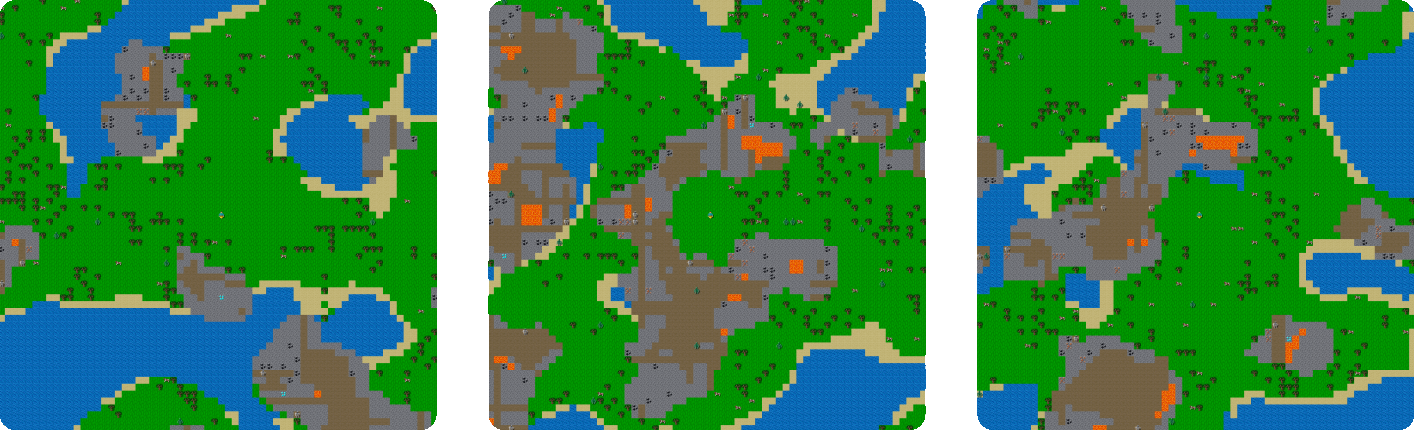
\includegraphics[width=1.0\textwidth]{iclr2025/images/crafter_map.png} 
    \caption{Crafter's examples of unique procedurally generated maps.}
    \label{fig:crafter_map} 
    \vspace{-2mm}
\end{figure}

\subsection{Crafter Results}
We provide Crafter results for LLM and VLM format in Tables \ref{crafter_LLM} and \ref{crafter_VLM}, standard errors are computed using 10 seeds. GPT4o leads in language-only mode, and Gemini-1.5-Pro leads in vision-language mode. Surprisingly, Llama 3.2 90B performance decreases very sharply when images are added, getting worse average progress than its smaller 11B model.

\begin{table}[h]
    \centering
    \begin{minipage}[t]{0.48\linewidth}
    \centering
    \caption{LLM Performance on crafter}
    \begin{tabular}{lc}
    \hline
    Model & Average Progress (\%) \\
    \hline
    gpt-4o & 33.10 $\pm$ 2.32 \\
    claude-3.5-sonnet & 32.73 $\pm$ 3.20 \\
    llama-3.2-90b-it & 31.68 $\pm$ 1.36 \\
    llama-3.1-70b-it & 31.21 $\pm$ 2.68 \\
    gemini-1.5-pro & 30.21 $\pm$ 2.86 \\
    claude-3.5-haiku & 26.36 $\pm$ 2.79 \\
    llama-3.2-11b-it & 26.19 $\pm$ 3.29 \\
    llama-3.1-8b-it & 25.45 $\pm$ 3.23 \\
    gemini-1.5-flash & 20.00 $\pm$ 0.74 \\
    llama-3.2-3b-it & 17.27 $\pm$ 2.79 \\
    gpt-4o-mini & 15.90 $\pm$ 2.05 \\
    llama-3.2-1b-it & 12.73 $\pm$ 1.91 \\
    \hline
    \label{crafter_LLM}
    \end{tabular}
    \end{minipage}
    \hfill
    \begin{minipage}[t]{0.48\linewidth}
    \centering
    \caption{VLM Performance on crafter}
    \begin{tabular}{lc}
    \hline
    Model & Average Progress (\%) \\
    \hline
    claude-3.5-sonnet & 37.27 $\pm$ 3.14 \\
    gemini-1.5-pro & 33.50 $\pm$ 2.07 \\
    gpt-4o & 26.81 $\pm$ 3.74 \\
    gemini-1.5-flash & 20.70 $\pm$ 4.42 \\
    gpt-4o-mini & 19.91 $\pm$ 3.13 \\
    llama-3.2-11b-it & 15.91 $\pm$ 1.16 \\
    llama-3.2-90b-it & 14.54 $\pm$ 1.80 \\
    \hline
    \label{crafter_VLM}
    \end{tabular}
\end{minipage}

\end{table}

\subsection{Observations}


\env{
You are an agent playing Crafter. The following are the only valid actions you can take in the game, followed by a short description of each action:
\newline\newline
Noop: do nothing,\newline
Move West: move west on flat ground,\newline
Move East: move east on flat ground,\newline
Move North: move north on flat ground,\newline
Move South: move south on flat ground,\newline
Do: Multiuse action to collect material, drink from lake and hit creature in front,\newline
Sleep: sleep when energy level is below maximum,\newline
Place Stone: place a stone in front,\newline
Place Table: place a table,\newline
Place Furnace: place a furnace,\newline
Place Plant: place a plant,\newline
Make Wood Pickaxe: craft a wood pickaxe with a nearby table and wood in inventory,\newline
Make Stone Pickaxe: craft a stone pickaxe with a nearby table, wood, and stone in inventory,\newline
Make Iron Pickaxe: craft an iron pickaxe with a nearby table and furnace, wood, coal, and iron in inventory,\newline
Make Wood Sword: craft a wood sword with a nearby table and wood in inventory,\newline
Make Stone Sword: craft a stone sword with a nearby table, wood, and stone in inventory,\newline
Make Iron Sword: craft an iron sword with a nearby table and furnace, wood, coal, and iron in inventory.\newline
\newline\newline
These are the game achievements you can get:\newline\newline
1. Collect Wood\newline
2. Place Table\newline
3. Eat Cow\newline
4. Collect Sampling\newline
5. Collect Drink\newline
6. Make Wood Pickaxe\newline
7. Make Wood Sword\newline
8. Place Plant\newline
9. Defeat Zombie\newline
10. Collect Stone\newline
11. Place Stone\newline
12. Eat Plant\newline
13. Defeat Skeleton\newline
14. Make Stone Pickaxe\newline
15. Make Stone Sword\newline
16. Wake Up\newline
17. Place Furnace\newline
18. Collect Coal\newline
19. Collect Iron\newline
20. Make Iron Pickaxe\newline
21. Make Iron Sword\newline
22. Collect Diamond\newline
\newline
In a moment I will present a history of actions and observations from the game.
Your goal is to get as far as possible by completing all the achievements.
\newline
PLAY!
}

\env[iclr2025/images/crafter.png]{Current Observation:\newline\newline
Your status:\newline
- health: 9/9\newline
- food: 9/9\newline
- drink: 9/9\newline
- energy: 9/9\newline
\newline
You have nothing in your inventory.\newline\newline
You see:\newline
- grass 1 steps to your west\newline
- tree 3 steps to your north-west\newline
- cow 3 steps to your west\newline\newline
You face grass at your front.\newline\newline
Image observation provided.
}

\agent{Move West}

\subsection{Analysis of VLM Performance in the Crafter Environment}

To investigate the agentic capabilities of VLMs in visually complex environments, we focused on the Crafter environment, a simplified 2D version of Minecraft. The environment uses tiled 2D textures to render scenes, which may be out-of-distribution for many VLMs. 
To address this potential limitation, we introduced an augmented version of the environment where scenes are rendered in 3D using Minecraft's 3D models and textures. This approach leverages data types more likely to be present in the training datasets of VLMs, given the abundance of interleaved text and images about Minecraft on the web.

\paragraph{Results} Surprisingly, the switch to 3D rendering did not improve VLM performance. In some cases, performance on the 3D-rendered environment was slightly worse than on the original 2D textures. This result challenges the hypothesis that familiarity with Minecraft-like 3D data in training datasets would lead to better performance. Instead, it suggests that VLMs may struggle with agentic tasks for reasons unrelated to the type of visual texture or rendering style.

\paragraph{Discussion} Our findings indicate that current VLM models may not be well-suited for complex vision-based reasoning tasks, even when provided with familiar visual contexts. The lack of improvement with 3D rendering suggests that factors other than texture familiarity, such as limitations in spatial reasoning or task-specific adaptation, may play a more significant role in their underperformance. While these preliminary results are insightful, further experimentation is necessary to draw stronger conclusions.


\begin{figure}[h] 
    \centering 
    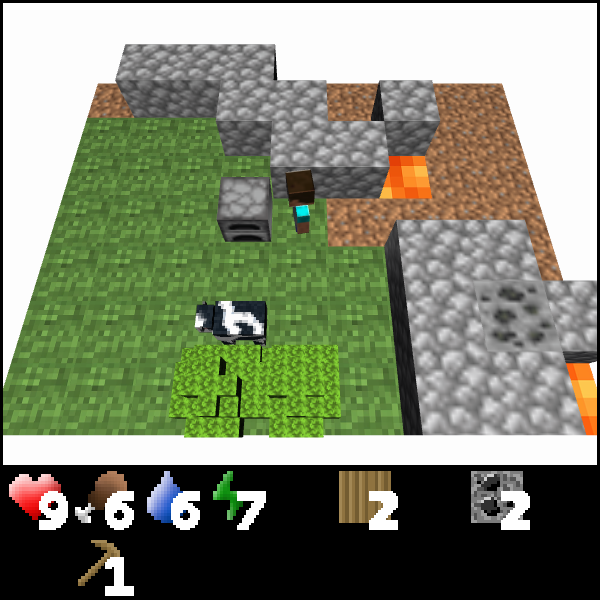
\includegraphics[width=0.6\textwidth]{iclr2025/images/crafter_render_3d.png} 
    \caption{Crafter's example of 3d scene visualization with Minecraft 3d models and textures.}
    \label{fig:crafter_3d} 
    \vspace{-2mm}
\end{figure}


\begin{table}[h]
\centering
\caption{Average Progress of VLMs in Crafter Across Rendering Types}
\begin{tabular}{lcc}
\hline
Model & 3d textures(\%) & 2d textures(\%) \\
\hline
claude-3.5-sonnet & 25.45 $\pm$ 4.18 &    37.27 $\pm$ 3.14 \\
gemini-1.5-pro & 30.45 $\pm$ 3.08 &      33.50 $\pm$ 2.07  \\
gpt-4o & 24.55 $\pm$ 3.65 &       26.81 $\pm$ 3.74  \\
gemini-1.5-flash & 19.09 $\pm$ 2.78 &   20.70 $\pm$ 4.43 \\
gpt-4o-mini & 17.27 $\pm$ 2.38 &       19.91 $\pm$ 3.13 \\
llama-3.2-11B-it & 15.90 $\pm$ 1.15 &     23.63 $\pm$ 1.48 \\
llama-3.2-90B-it & 12.27 $\pm$ 1.44 &    10.00 $\pm$ 1.13 \\
\hline
\end{tabular}
\label{Crafter_Ablation}
\end{table}
